 \documentclass{article} %A4
\usepackage[a4paper,left=1.9cm, right=2.1cm,top = 1.2cm,bottom=2.3cm]{geometry}
\usepackage[utf8]{inputenc}%Umlaute
\usepackage[ngerman]{babel} %Texttrennung
\usepackage{graphicx}	%Grafiken
\usepackage{amssymb}
\usepackage{amsmath}
\usepackage{url}
\usepackage{listings}
 \usepackage{color}
\usepackage{hyperref}
\usepackage{framed}
\usepackage{algpseudocode}
\usepackage{tikz}

\usepackage[labelformat=empty]{caption}
\title{Zusammenfassung - Kryptographie}
\author{
	Marc Meier
}

\begin{document}
\maketitle
\begin{framed}Korrektheit und Vollständigkeit der Informationen sind nicht gewährleistet.
Macht euch eigene Notizen oder ergänzt/korrigiert meine Ausführungen!
\end{framed}
\setcounter{tocdepth}{1}
\tableofcontents

\begin{framed}
Planung der Veranstaltung % Kann später wahrscheinlich ausgelassen werden.
\begin{enumerate}
	\item Wiederholung (ca 3-4 Termine)
	\begin{itemize}
		\item Probleme, Kodierung von Problemen, Laufzeit von Algorithmen
		\item P, PN, NPC…
		\item Grundlegende Probleme \& Algorithmen
	\end{itemize}
	\item Algorithmen für schwierige Probleme (ca. 15 Termine)
	\begin{itemize}
		\item parallele / randomisierte Algorithmen
		\item Approximationsalgorithmen
		\item parametrisierte Algorithmen
	\end{itemize}
	\item Kryptographie (ca 10 Termine)
	\begin{itemize}
		\item Public-Key-Kryptographie
	\end{itemize}
\end{enumerate}
\end{framed}
\section{Grundlagen und Wiederholungen}
\subsection{Probleme, deren Kodierung und Laufzeit von Algorithmen}
Anhand einiger Beispiele soll die Wichtigkeit der Kodierung der Probleme bzw. der Eingabe verdeutlicht werden.
\subsubsection{Sortieren}
\begin{description}
	\item[Eingabemenge:] Natürliche Zahlen $a_1, a_2,...,a_n$
	\item[Ausgabe:] Eingabe aufsteigend sortiert
\end{description}
Beim Sortieren handelt es sich um ein \emph{Suchproblem}.
Beispiele für bekannte Sortieralgorithmen und deren Laufzeitkomplexität sind Bubblesort $\mathcal{O}(n^2)$ und Mergesort $\mathcal{O}(n\log{}n)$\footnote{Sofern nicht anders angegeben entspricht $\log n$ immer dem dualen Logarithmus von n (Basis 2)}.
\subsubsection{Eingabelänge N}
Die Länge der Eingabe entspricht \emph{nicht} der Anzahl der zu sortierenden Elemente $n$.
Dies ist aufgrund der Kodierung in eine maschinenlesbare Form der Fall.
Für gewöhnlich verwenden heutige Computer eine Darstellung im Binärsystem. Daher gilt:
\begin{equation}
N := \sum_{i=1}^n \log a_i
\end{equation}
Im Folgenden soll die Eingabe [11, 13, 113] kodiert werden.
Für eine Turingmaschine mit dem Eingabealphabet $\Sigma := \{0,1,\$ \}$ würde diese folgendermaßen aussehen:
1011\textbf{\$}1101\textbf{\$}1110001.
Um eine Lesbarkeit für Binärrechner zu ermöglichen, werden weiterhin folgende Ersetzungen durchgeführt:
$1 \rightarrow 11$
$0 \rightarrow 00$
$\$ \rightarrow 01$
Die resultierende Kodierung wäre nun:
11001111\textbf{01}11110011\textbf{01}11111100000011.
Sei nun $L$ die maximale Wortlänge\footnote{An dieser Stelle habe ich mit Förmi geschnattert und weiß daher nicht, ob das so korrekt ist}.
\begin{equation}
L := max_{i=1}^n \log a_i
\end{equation}
Hier sollte ergänzt werden, wie man auf das $\mathcal{O}(N^3)$ kommt.

\subsubsection{Primzahl}
\begin{description}
	\item[Eingabemenge:] Eine natürliche Zahl $n$
	\item[Ausgabe:] Ist $n$ eine Primzahl? 
\end{description}
Es handelt sich um ein \emph{Entscheidungsproblem}.
Die Eingabelänge ist $N := \log n$.
Ein naiver Algorithmus wird im Folgenden beschrieben.

\begin{algorithmic}[1]
	\If {$n = 2$} \State \Return Ja
	\Else \For {$d:=2$ \textbf{to} $n-1$}
		\If {$n \mod d = 0$}
			\State \Return Nein
		\Else
		\EndIf
	\EndFor
	\State \Return Ja
	\EndIf
\end{algorithmic}

Die Komplexität lässt sich wie folgt herleiten:
Für die Verzweigungen (Zeilen 1 und 5), sowie für die return-Statements in den Zeilen 2 und 6 ist eine beschränkte Komplexität $\mathcal{O}(1)$ anzunehmen.
Alle Statements in der for-Schleife werden $n-2$ mal wiederholt, die Komplexität ist $\mathcal{O}(n)$.

Die daraus resultierende Komplexität $\mathcal{O}(n)$ ist äquivalent zu $\mathcal{O}(2^{\log n})$.
Weil $\log n$ der Eingabelänge N entspricht, ist die Komplexität entsprechend $\mathcal{O}(2^N)$, also exponentiell.
Demnach ist der Algorithmus nicht effizient.

\subsubsection{Cliquensuche im Graphen}

\begin{framed}
\textbf{CLIQUE}\\
\begin{description}
	\item[Eingabemenge:] Graph $G= (V,E)$ und $k \in N$
	\item[Ausgabe:] Hat G mindestens paarweise verbundene Knoten (eine Clique C mit $\geq k$ Knoten)?
\end{description} 
\end{framed}

\begin{framed}
\textbf{CLIQUE (Suchproblem)}\\
\begin{description}
	\item[Eingabemenge:] Graph $G= (V,E)$
	\item[Ausgabe:] !!!!!!!!!!!!!!ERGÄNZEN!!!!!!!!!!!!!!!!
\end{description} 
\end{framed}

\textbf{Behauptung:} Wenn CLIQUE (Entscheidungsproblem) in polynomieller Zeit lösbar ist, so ist auch die Suchversion von CLIQUE in polynomieller Zeit lösbar.\footnote{In polynomieller Zeit, abhängig von der Knotenzahl $|V|$ des Graphen}

\textbf{Beweis}
\begin{description}
\item[$\Leftarrow$] Zur Eingabe (G,k) von CLIQUE  bestimmen wir zunächst mit dem Algorithmus für CLIQUE-Suchversion eine größte Clique C von G.
Es wird verglichen, ob $|C| \geq k$ gilt.
Ist dies der Fall, gibt der Algorithmus \emph{Ja} zurück, andernfalls \emph{Nein}.
Die Laufzeit entspricht offensichtlich der Clique-Suchversion.

\item[$\Rightarrow$] Betrachte folgende Zwischenversion für CLIQUE:
Betrachte folgende Zwischenversion für CLIQUE\footnote{$\omega(G) = max \{|C|: C$ ist eine Clique in $G\}$ ist die Cliquenzahl}:
\begin{framed}
\textbf{CLIQUE-Zwischenversion:}
\begin{description}
\item  [Eingabe:]Graph G=(V,E)
\item [Aufgabe:] Bestimme die Maximalzahl $\omega (G)$  von paarweise verbundenen Knoten in G
\end{description}
\end{framed}
\end{description}
\textbf{Behauptung:} CLIQUE in polynomieller Zeit lösbar $\Rightarrow^{(1)}$ CLIQUE-Zwischenversion in polynomieller Zeit $\Rightarrow^{(2)}$ CLIQUE-Suchversion in polynomieller Zeit lösbar.

\begin{description}
\item[zu (1):] Sei A ein Algorithmus für CLIQUE in polynomieller Zeit.
Zur Eingabe G von CLIQUE-Zwischenversion wende A auf Eingaben $(G,n), (G,n-1),...,(G,1)$ an!
Ausgabe ist $\omega (G) =$ erstes k mit $A(G,k) = Ja$

\begin{algorithmic}[1]
\For{ k:= n to 1}
	\If A(G,k) = 'ja'
	then return $\omega (G) = k $
	\EndIf
\EndFor
\end{algorithmic}
Laufzeit: $n \cdot \mathcal{O}(n^c) = \mathcal{O}(n^{c+1})$


\item[zu (2):]: Sei A ein polyzeit Algorithmus für Clique-Zwischenversion.
d.h. $A(G) = \omega (G)$ in $\mathcal{O}(n^d)$ für eine Konstante d.

Zur Eingabe G von Clique-Suchversion wende folgendes an:
\begin{algorithmic}[1]
\For {jede Kante $e \in E$ }
	\If{ $\omega (G - e ) = \omega (G)$}
	 $G := G - e$
	\EndIf
\EndFor
\State \Return {C := V(G) ohne isolierte Knoten}
\end{algorithmic}
\end{description}


\begin{table}[h]
\centering
\begin{tabular}{|l|l|l|p{8cm}|}
\hline
$G$ &  $\omega (G) = 3$ & 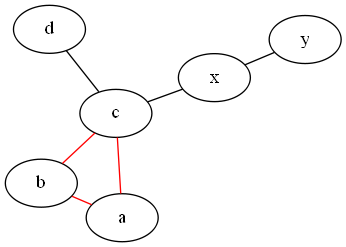
\includegraphics[width=0.2\textwidth,trim=0 0 0 -5]{img/clique1.png} &   Vollständiger Graph \\ \hline
$G_2 := G - cx$ &  $\omega (G) = 3$ & 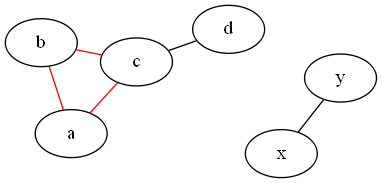
\includegraphics[width=0.2\textwidth,trim=0 0 0 -5]{img/clique2.png} & Nach Entfernen der Kante \emph{cx} hat sich die Cliquenzahl nicht geändert, die Knoten x und y sind isoliert.
Die Kante \emph{ex} ist also nicht für die Clique notwendig. \\ \hline
$G_3 := G_2 - bc $  & $\omega (G) = 2$  & 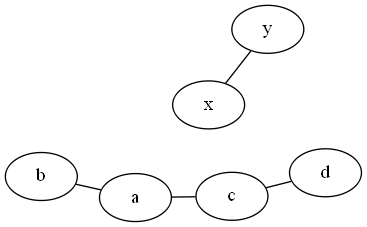
\includegraphics[width=0.2\textwidth,trim=0 0 0 -5]{img/clique4.png} & Nach Entfernen der Kante \emph{bc} hat sich die Cliquenzahl verringert.
 Offensichtlich wird \emph{bc} also für die Clique benötigt. \\ \hline
$C := \{a,b,c\} $  & $\omega (G) = 3$  & 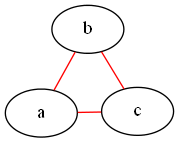
\includegraphics[width=0.2\textwidth,trim=0 0 0 -5]{img/clique3.png} & Im weiteren Verlauf wird (offensichtlich) noch die Kante \emph{cd} entfernt. Anschließend werden die isolierten Knoten d, x und y entfernt und die Lösung $C := \{a,b,c\}$ zurückgegeben.\\ \hline
\end{tabular}
\end{table}

\textbf{Hinweis:} Ich bin mir nicht sicher, ob es sich um das korrekte Beispiel aus der Vorlesung handelt.\\

\textbf{Laufzeit:} $m \cdot \mathcal{O}(n^d) = \mathcal{O}(n^{d+2})$

\subsubsection {Gegenüberstellung \glqq einfache Formulierung\grqq {} vs \glqq formale Formulierung\grqq}
Die genaue Formulierung des Problems ist wichtig:

\glqq Ist n prim?\grqq

genauer:
 
\begin{description}
	\item[Eingabemenge:] Eine natürliche Zahl $n$
	\item[Ausgabe:] Ist $n$ eine Primzahl? 
	\item [Formal:] $PRIM \footnote{bin(n) - Binärdarstellung von n} = \{ bin(n) |  n \in N$ ist prim$\} \subset \{0,1\}^+$
\end{description}


Venn-Diagramm $PRIM \subset \{0,1\}^+$ TODO (Und offensichtlich falsch, da ich noch keinen Plan von TIKZ habe)
\def\firstcircle{(0,0) circle (1.5cm)}
\def\secondcircle{(45:2cm) circle (1.5cm)}

% Now we can draw the sets:
\begin{tikzpicture}
    \draw \firstcircle node[below] {$ \{0,1\}^+$};
    \draw \secondcircle node [above] {$PRIM$};


    \begin{scope}
      \clip \firstcircle;
      \fill[red] \secondcircle;
    \end{scope}


\end{tikzpicture}


\subsection{ P, PN, NPC}
P = Menge aller \emph{Entscheidungsprobleme}, für die ein (deterministischer) polynomialzeit-Algorithmus existiert (formal via Deterministischer Turing Maschine, \glqq effizient lösbare Probleme\grqq).
Ein \emph{Optimierungsproblem} ist lösbar, wenn die entsprechende Entscheidungsversion in P ist.

\subsubsection{Grundlegende Probleme in P}
\begin{itemize}
\item\textbf{Sortieren}
\item\textbf{PRIM} - Allerdings nicht der vorgestellte Algorithmus. Effizienter Algorithmus wurde 2002 vorgestellt. Komplexität $\mathcal{O}(\log n)^{12})$, zur Zeit sogar $\mathcal{O}(\log n)^{6})$\url{ https://de.wikipedia.org/wiki/AKS-Primzahltest}
\item\textbf{2-SAT}  (Modellierung mit Graphenproblem für Beweis)
\end{itemize}

\bibliographystyle{alpha}
\bibliography{literatur}

\begin{framed}
\textbf{Übrige Notizen}

In der Praxis ermittelt man die Komplexität der Einfachheit halber mit uniformen Kostenmaß.
Sortierung:
Eingabe: $a_1, a_2,...,a_n$ beziehungsweise $bin(a_1) \# bin(a_2) \# ... \# bin(a_n) $ mit Ersetzung 
Aufgabe: Sortiere Zahlen aufsteigend
Mergesort: $\mathcal{O}(n \cdot \log n)$
Problem -> Eingabelänge (siehe oben, hatten wir schon)
\end{framed}
\end{document}